% API Hierarchy for MuSyCo-ArEx.
% Author: J. Korinth (TU Darmstadt), jk@esa.cs.tu-darmstadt.de
\documentclass[border=2pt,varwidth,10pt]{standalone}
\usepackage{tikz}
\usetikzlibrary{patterns,calc,backgrounds}
\renewcommand\rmdefault{\sfdefault}
% define simple color names for esa colors and a highlight
\definecolor{esa}{RGB}{10,156,215}
\def\esacolorfactor{20}
\colorlet{esa0}{esa!90!white}
\colorlet{esa1}{black!\esacolorfactor!esa0}
\colorlet{esa2}{black!\esacolorfactor!esa1}
\colorlet{esa3}{black!\esacolorfactor!esa2}
\colorlet{esa4}{black!\esacolorfactor!esa3}
\colorlet{esa5}{black!\esacolorfactor!esa4}
\definecolor{highlight}{RGB}{189,27,27}



\begin{document}
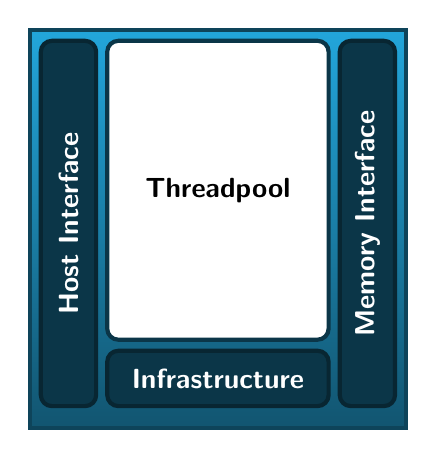
\begin{tikzpicture}[line width=1.5pt,
    platform background/.style={fill=esa5, draw=black!30!esa5, rounded corners},
    arch background/.style={fill=white, draw=esa5, rounded corners}
  ]
  \def\height{132pt}
  \def\archwidth{80pt}
  \def\sidewidth{20pt}
  \def\xgw{4pt}
  \def\ygw{\xgw}
  \def\botheight{\sidewidth}
  \coordinate (c) at (0,0);
  \coordinate (al) at (-.5*\archwidth,0);
  \coordinate (ar) at (.5*\archwidth,0);
  \coordinate (hl) at (-.5*\archwidth - \sidewidth - \xgw,0);
  \coordinate (hr) at (-.5*\archwidth - \xgw,0);
  \coordinate (ml) at (.5*\archwidth + \xgw,0);
  \coordinate (mr) at (.5*\archwidth + \sidewidth + \xgw,0);

  \coordinate (t) at (0,0);
  \coordinate (b) at (0, -\height);
  \coordinate (ab) at (0, -\height + \botheight + \ygw);
  \coordinate (it) at (0, -\height + \botheight);

  \begin{scope}[every path/.style={platform background}, every node/.style={font=\bfseries\color{white}}]
    \path (hl |- t) rectangle (hr |- b) node [pos=0.5, rotate=90] {Host Interface};
    \path (ml |- t) rectangle (mr |- b) node [pos=0.5, rotate=90] {Memory Interface};
    \path (al |- it) rectangle (ar |- b) node [pos=0.5] {Infrastructure};
  \end{scope}
  \path [arch background] (al |- t) rectangle (ar |- ab) node [pos=0.5, font=\bfseries\color{black}] {Threadpool};

  \begin{pgfonlayer}{background}
    \shade [top color=esa0, bottom color=esa3, draw=esa4, line width=1.5pt] (hl |- t) +(-\xgw, \ygw) rectangle ($(mr |- b) +(\xgw, -2*\ygw)$);
  \end{pgfonlayer}
\end{tikzpicture}
\end{document}
